
\chapter{Background}

\label{ch:background}

\section{Introduction} 

Interactive tables are by no means a new idea. A lot of research has
been undertaken to find a simple suitable solution for the problem.

\subsection{Huddle Lamp} \label{Sec:huddlelamp}
\begin{figure}[H]
\centering
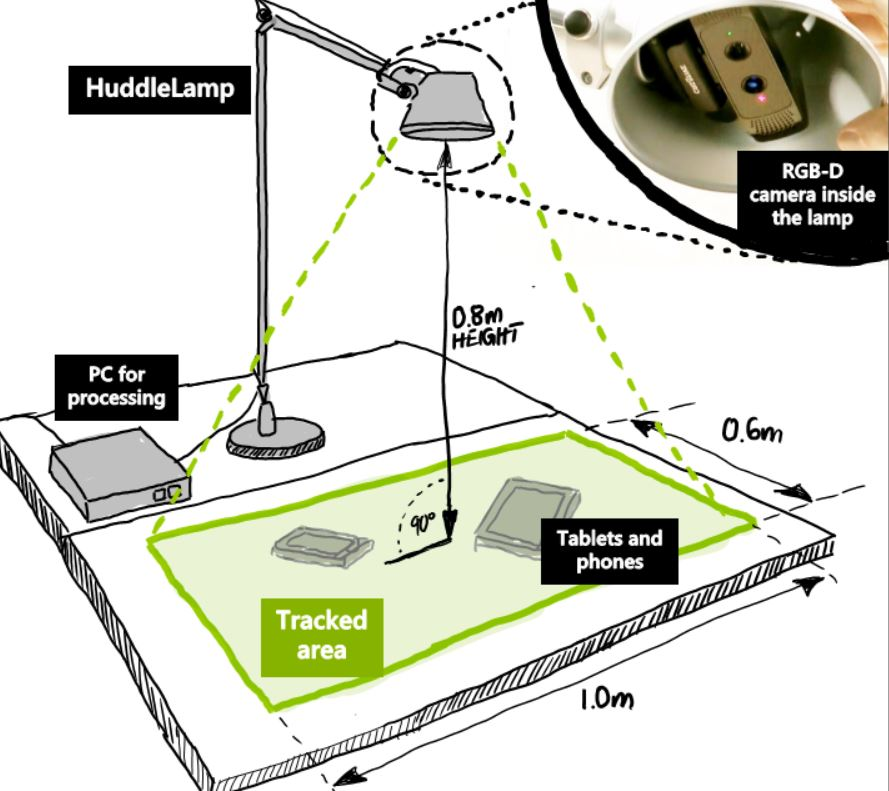
\includegraphics[scale=0.4]{huddlelamp_setting}
\protect\caption{HuddleLamp Setting}
\end{figure}
HuddleLamp aims to use the multitude of unused tablets and smart-phones,
which people have lying around to, create an ad-hoc interactive table
by using a novel sensing and detection method to deduce where the
devices are and what they should be show. The research into HuddleLamp\cite{huddle-link}, is the work that
is most similar to mine. HuddleLamp is trying to bring the option of having interactive tables to a wider market. Currently every day consumers such as schools and public libraries find it difficult to install an interactive table.


HuddleLamp\cite{huddlelamp-paper} proposes to use some cheaper
off-the-shelf products like a web cam, and a lamp fixture to create a cheaper
interactive table that anyone could use. HuddleLamp\cite{huddlelamp-paper} introduces a hybrid sensing approach that uses RGB (the red, green and blue light information for each pixel) and depth data, that can be obtained from sophisticated webcams like the Creative senz3d\cite{creative-senz3d}, which can detect and identify mobile displays on tables and track their positions and orientations. The project attempts to provide a way for multiple devices to interact with each other and become one seamless multi-device user interface.

One of the main advantages of HuddleLamp was the fact that you can add a device onto the user interface (UI) in a seam-less, ad-hoc manner. Using HuddleLamp,
users can add or remove displays and reconfigure them in the space without
the need for installing any software or attaching markers. Placing
devices below the camera implicitly does the setup and pairing.
Opening a URL on the device and making it visible to the camera adds
the new device to the \textquotedblleft Huddle\textquotedblright .
The camera also tracks the hand movements of the user, enabling interactions
between the devices.

The simplicity in adding a device to the table means users are not
constrained by having specific devices or requiring them to download
particular apps. This also means collaboration can occur on tables
that are cluttered with other objects likes pens and pencils. There
are 2 main components that are required for HuddleLamp;
a depth camera, they suggest Creative Senz3D\cite{creative-senz3d} camera, and a desk lamp, both
are relatively inexpensive components compared to an interactive table.

However there are some deficiencies in this system that makes
an interactive table. At the time of writing, the project has not
released a public version of their software. The developer
version requires you to connect a computer with the web cam, which
does most of the work in term tracking devices and gesture recognition. In this architecture
of HuddleLamp, the computer does all the resource intensive tasks so if it is
not a really powerful computer, users could experience a delay. The fact
that to set this interactive table up you need to connect a lamp up
to a computer means that the whole setup is not very portable. The
size of the interactive part of the table is constrained by how high
up the camera is, from the surface of the table. The use of a camera
means users arms and hands can sometimes impede the
detection and tracking of devices during moving or touching the devices.
Also the suggested camera and its software development kit (SDK) required
for the project has been taken off the market by its producer. Making
it imperative that an alternative to HuddleLamp is identified.

\subsection{ConnecTable}

ConnecTable\cite{connectables} was one of the first attempt at creating
an interactive table. It is a mobile, context aware
information appliance, which uses a pen-based interaction. It uses
dynamic, flexible coupling of displays to circumvent the limitation
of display real estate. By using in built sensors it has the ability
to merge displays, when they come together, to form a homogeneous physical
display. When 2 or more ConnecTables are connected, users are able
to exchange information by shuffling them over to the other display.
It predominantly has a pen based interaction, however it also provides sensors
integrated onto the tabletop that translate physical actions in the
real world to interactions on the tables. 
\begin{figure}[H]
\centering
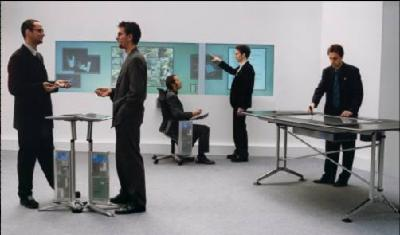
\includegraphics[scale=0.5]{connectables}

\protect\caption{ConnecTable Configuration}
\end{figure}
ConnecTable uses the movement in real space and engagement in discussions
between users as cues on when to connect with other tables. It also
has multiple use modes where two tables could connect together to
become a homogeneous display, or it could connect together to have
two simultaneous displays, allowing both users to see and interact on
the same object in different screens, similar to group collaboration
in a Google Doc. ConnecTable uses transponders based on radio frequency
technology and electromagnetic waves for its sensing technology. The
table has a coil which emits an electromagnetic wave and a transponder
from the connecting table sends its 32 bit identification number
back to the initiating table. The identification mechanism works in
a range of around 3cm and takes nearly 1.5 seconds to complete.

\todo[inline]{disadvantages}

\begin{figure}[h]
\centering
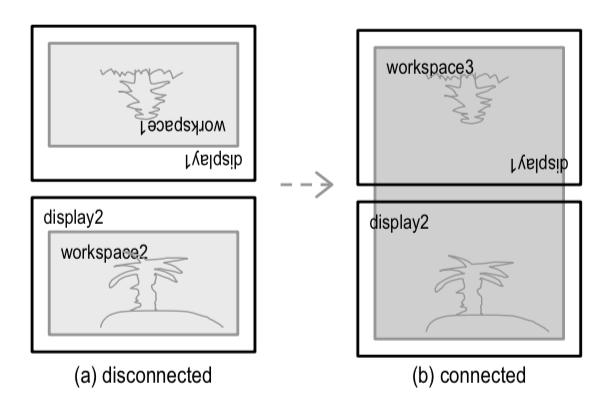
\includegraphics[scale=0.5]{connecTable_views}
\protect\caption{Shows the difference in views between connected and disconnected ConnecTables}
\end{figure}

\subsection{Beamatron} \label{beamatron}

Beamatron \cite{beamatron} is a contribution by Microsoft research,
in to the fields of Spatial Augmented Reality. It uses depth cameras
with proprietary algorithms and techniques to render graphics precisely
onto the real world according to the user's point of view. By using a
depth camera they were able to add more modes of interaction to augmented
reality, i.e moving objects or holding onto an object. It has the capabilities
to allow live changes on the projections. It can reason with room
coordinates and render 3D objects in precise orientation and also uses 3D
sound source localisation as a means to track user position when the
user is not in view. 
\begin{figure}
\centering
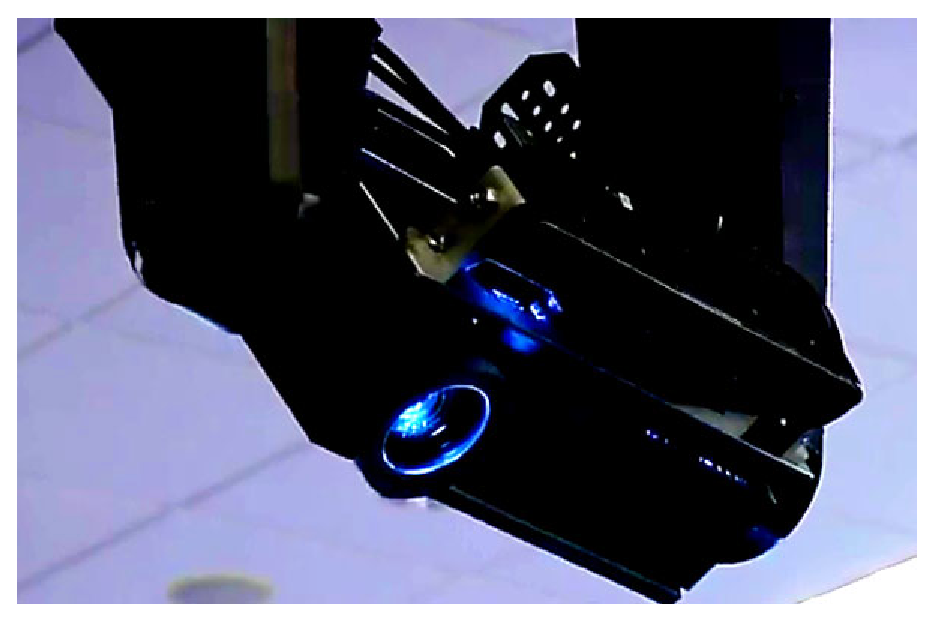
\includegraphics[scale=0.3]{Microsoft_Kinect_AR_Beamatron}
\protect\caption{Beamatron}
\end{figure}
Beamatron hardware consist of a video projector and a Microsoft XBox
Kinect sensor mounted to a City Theatrical Autoyoke\cite{autoyoke}
moving light platform. To get the information about the pan and tilt
of the Autoyoke they had to create a bespoke circuit board which connected
to the respective encoders of the Autoyoke giving Beamatron accurate
hardware-based feedback which allowed graphics to be stabilised. 

One of the biggest shortcomings of placing a steerable display in
the centre of the room is that the information received is limited
to the view of the single camera. They compensated for the lack of
depth information by mounting multiple 3 Kinect sensors to the corners
of the room and using triangulation to find sources of sound and in
turn identifying the presence of the user. They reported some shortcomings
in their technique, failures occurred especially when the user is standing beneath the
Beamatron.
The ideas and technique explored for Beamatron were intriguing. Especially
the positioning technique they used to locate the user when not in
the view of the depth camera. However the use of multiple Kinect sensors
and projector fixed to the centre of the view meant that the apparatus
was not portable. There was also quite a difficult calibration method
required.


\subsection{LightSpace}
\begin{figure}[H]
\centering
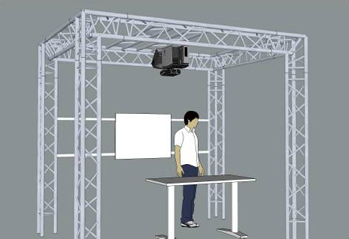
\includegraphics{LightSpace_configuration}
\protect\caption{LightSpace Configuration}
\label{lightspace-config}
\end{figure}

LightSpace is another research contribution by Microsoft in the "smart-room" field of research\cite{lightspace}. LightSpace is an office-sized room instrumented with projectors and depth cameras. These instruments combine together to help the user to touch and manipulate virtual objects that are in the room, on un-instrumented surfaces. The depth camera aids to determine the location of users hand by doing real-time 3d surface geometry. Some of the main motivation for the LightSpace project was to have: 
\emph{Surface Everywhere} where all physical surface should be interactive displays, 
\emph{The room is the computer} even the space between the physical surface should be interactive and 
\emph{Body as display} graphics may be projected in onto the user's body to enable interactions such as holding and carrying the object.
Their primary target was to enable interactivity and visual- izations throughout our everyday environment, without augmenting users and other objects in the room with sensors or markers\cite{lightspace}.

The LightSpace implementation is  a 10ft (W) x 8ft (D) x 9ft (H) interactive space in which we suspended 3 projectors and 3 depth cameras together from the ceiling (Figure \ref{lightspace-config})\cite{lightspace}.

This project is quite similar to the Section \nameref{beamatron} project however LightSpace has a bigger field of vision due to its multiple projectors and depth cameras. LightSpace has made major breakthroughs in terms of converting 3D space into interactive space and also in terms of adding multiple interactions to a room. However this project is more useful for someone creating a smart room. Information about using vision manipulation could help for HuddleTable, however this an implementation that is fixed to an area and cannot be moved, which goes against my idea of having a very portable product that could be set up anywhere. 

\subsection{SufacePhone}

SurfacePhone\cite{surfacephone} is a research concept which used
a projector in conjunction with a mobile device to project onto a
physical surface to allow a tabletop like interaction in a mobile setup.
It has touch and gesture interaction incorporated giving a
realistic user experience. As the computing power of the mobile devices have
increased and now rivals a desktop, users wants to do increasingly complex
tasks on their mobile devices. However one of the main limitation
of mobile devices are their display size. 

SurfacePhone comes with a multitude of configurations. It could be
used as Single-device, Single User (SDSU) or the projections can merge
when multiple devices comes into proximity to make a Multi-device,
multi user interaction (MDMU) which creates a larger shared surface. 

Some of the troubles they came across with the devices was the actual
hardware. Since it required both a mobile device and projector, it
was a rather expensive tool to carry around with. Adding the projector
onto the phone meant the device was quite big and inconvenient to carry around. There was also
trouble with getting some aspects of interactions to work such as
Multi-modal touch.
\begin{figure}[H]
\centering
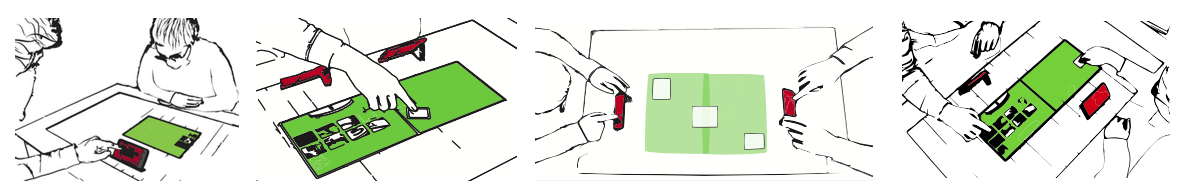
\includegraphics[scale=0.25]{surfacePhone}

\protect\caption{SurfacePhone}


\end{figure}

